\section{Lab setup and scenarios}
\label{sec:lab_setup_and_scenarios}
In this section, the setup of the experiments is described, including the network configuration, the hardware and the software utilized.

\subsection{Hardware}
The hardware used for the experiments includes:

\begin{itemize}
    \item \textbf{Host A} \label{sec:host-a}:
        \begin{itemize}
            \item Product name: Acer Nitro 5 AN515-55
            \item Ethernet interface: Intel{\textregistered} Killer{\texttrademark} Gigabit Ethernet E2600
            \item Wireless interface: Intel{\textregistered} Wi-Fi 6 AX201 160MHz (802.11ax) 2x2
            \item Operating system: Ubuntu 22.04.4 LTS
        \end{itemize}
    \item \textbf{Host B} \label{sec:host-b}:    
     \begin{itemize}
            \item Product name: Apple MacBook Pro 13" 2019 
            \item Ethernet interface: Rankie USB3.0 to Gigabit Ethernet Adapter
            \item Wireless interface: Broadcom BCM4377b Wi-Fi 5 80MHz (802.11ac) 2x2
            \item Operating system: MacOS Sonoma 14.0
        \end{itemize}
    \item  \textbf{Router}: 
        \begin{itemize}
            \item Product name: iliadbox with Wi-Fi 5 technology
            \item Ethernet interface: 1 Gbps LAN port
            \item Wireless interface: WiFi 11n 2x2 2.4GHz, 11ac 4x4 5GHz
        \end{itemize}
    \item \textbf{Ethernet} cable: UTP Cat6, 1 Gbps
\end{itemize}

The network experiments configurations are the following:

\begin{itemize}
    \item \textbf{Ethernet Link}:
    \begin{itemize}
        \item Protocol: 802.3ab (1000BASE‑T Full duplex)
        \item Nominal link speed: 1 Gbps
    \end{itemize}

     \item \textbf{WiFi Link}: 
     \begin{itemize}
         \item Protocol: 802.11ac
         \item Frequency Band: 5 GHz
         \item Bandwidth: 80 MHz
         \item Channel: 44
         \item Nominal link speed: 867 Mbps
         \item Number of connected stations: 6
         \item Security protocol: WPA2-AES
     \end{itemize}
\end{itemize}
In the figure \ref{fig:channel_occupation_and_noise} it is possible to notice that the Wi-Fi channel used by the access point during the tests (channel 44) does not have an high noise level and it has a low occupation rate.

\begin{figure}[H]
\centering
\vspace{-30pt} 
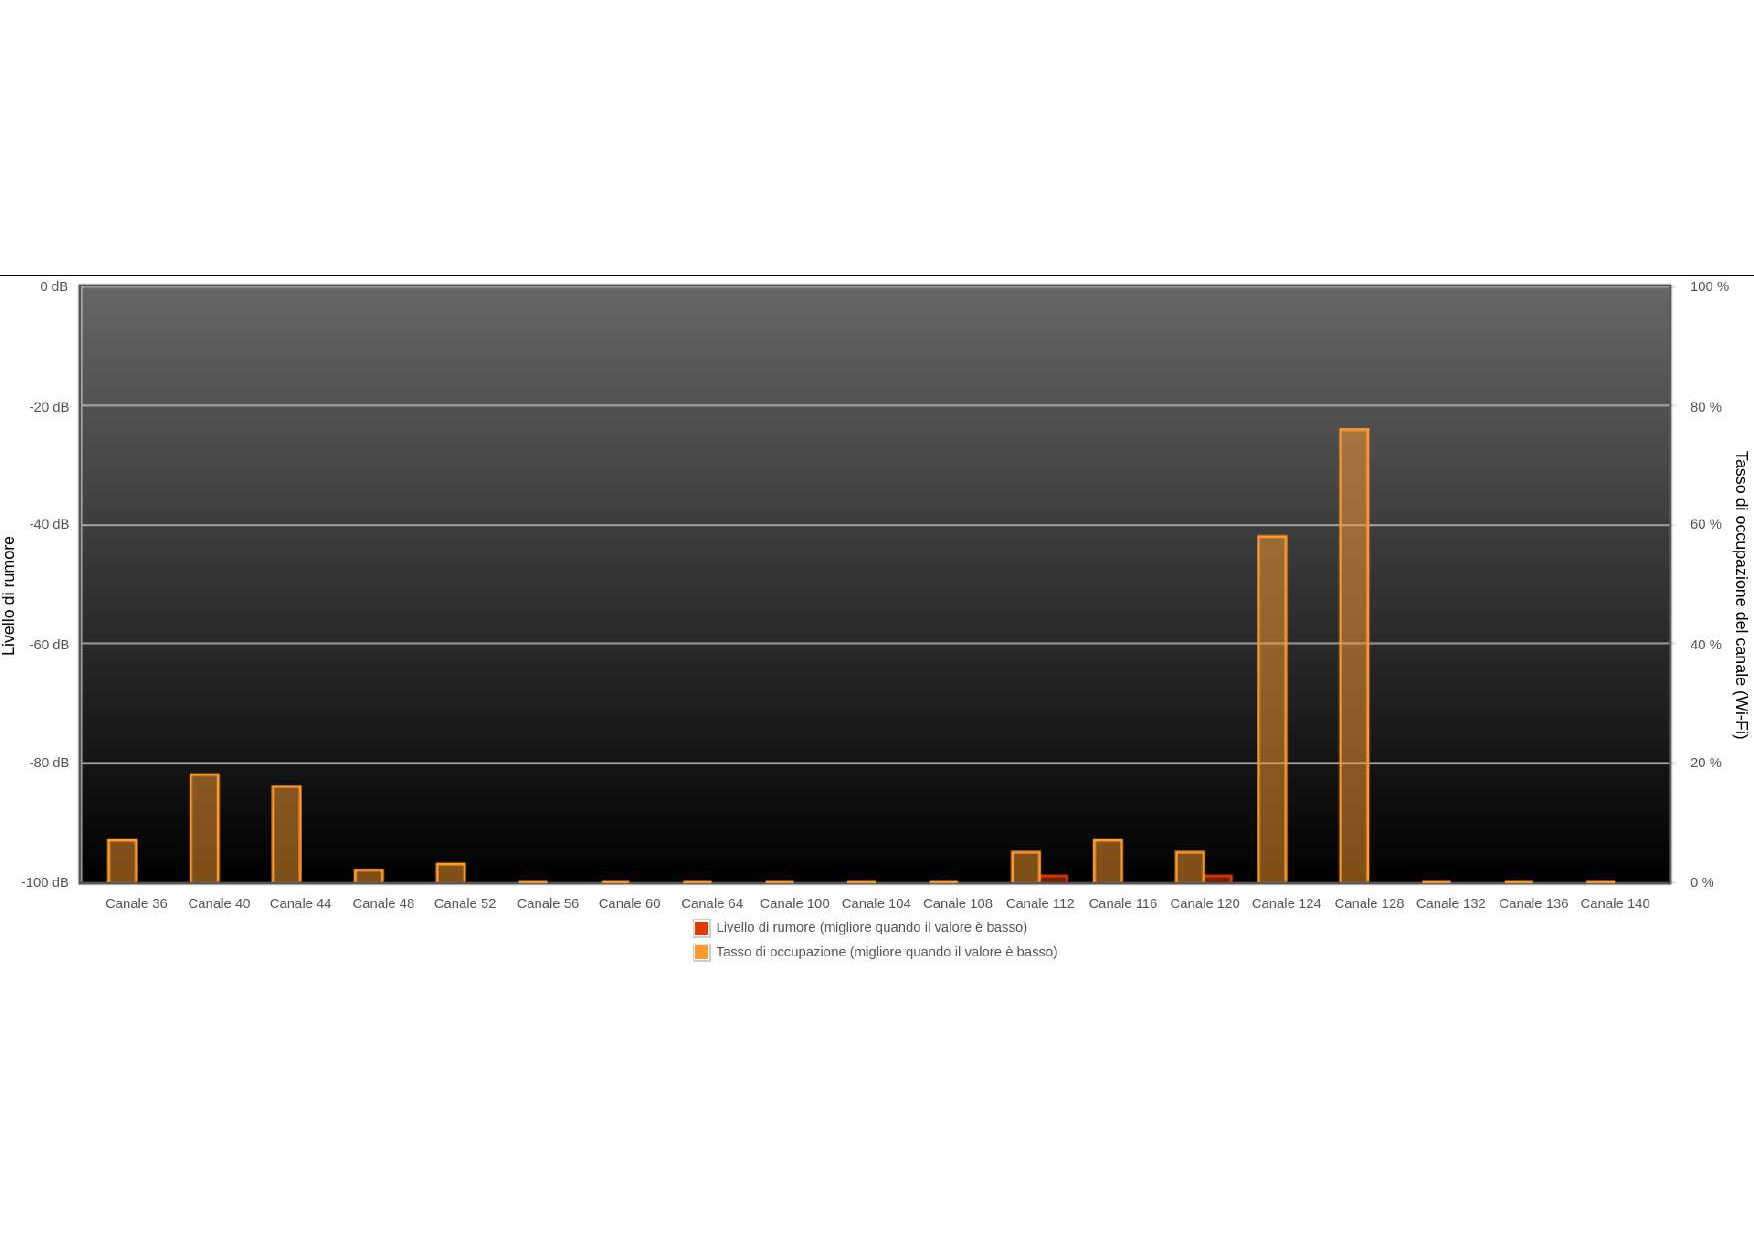
\includegraphics[width=0.5\textwidth]{images/channel_occupation_and_noise.pdf}
\vspace{-50pt} 
\caption{5GHz band occupation and noise}
\label{fig:channel_occupation_and_noise}
\end{figure}
\vspace{-5pt}
    
\subsection{Scenarios}
The tests scenario are the following:
\begin{itemize}
    \item \textbf{Both Ethernet}: Host A and Host B are directly connected trough the Ethernet cable
    \item \textbf{Both Wi-Fi}: Host A and Host B are connected to the same Wi-Fi network
    \item \textbf{Mixed}: The Host A is connected to the Router using the Ethernet cable, the Host B is connected to the Router Wi-Fi network
\end{itemize}

\vspace{-15pt}
\begin{figure}[H]
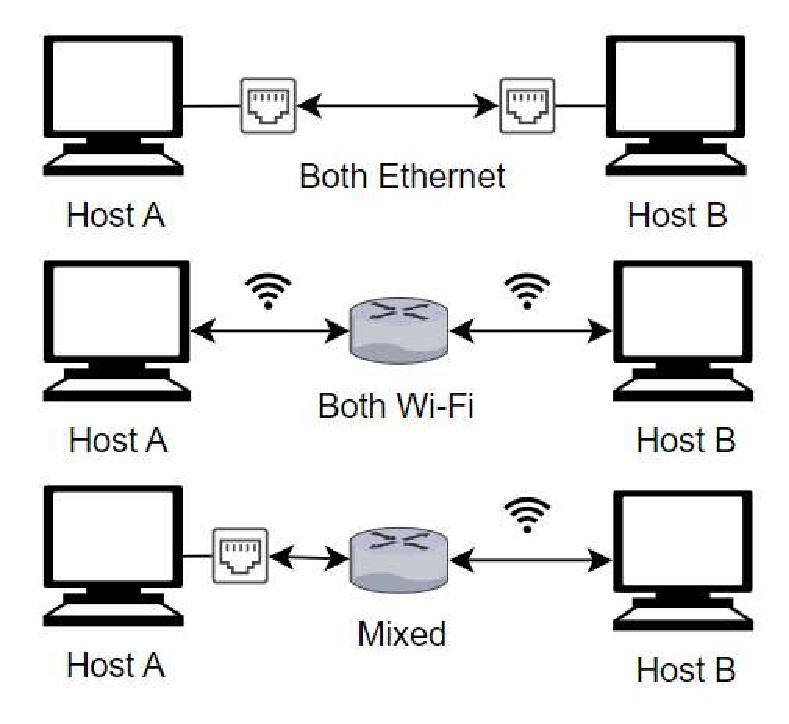
\includegraphics[scale=0.25]{images/setup_scenarios.pdf}
\vspace{-10pt}
\caption{Setup scenarios}
\label{fig:setup_scenarios}
\end{figure}
The expected goodputs, in the different scenario are (C is the capacity of the bottleneck link): 
\begin{itemize}
    \item Both Ethernet
    \begin{itemize}
        \item TCP: $ G \leq \eta_{TCP_{Eth}} * C_{Eth} = 94.9\% * 1000 Mbps = 949 Mbps $ 
        \item UDP: $ G \leq \eta_{UDP_{Eth}} * C_{Eth} = 95.7\% * 1000 Mbps = 957 Mbps $  
    \end{itemize}

    \item Both WiFi: since both \hyperref[sec:host-a]{Host A} and \hyperref[sec:host-b]{Host B} have 2x2 wireless cards (so 2 spatial streams), then the maximum bitrate (for a 80MHz channel) is for both hosts 867 Mbps~\cite{802.11ac_data_rates_and_speed}. Furthermore, since the medium is shared and half duplex, and since \hyperref[sec:host-a]{Host A} and \hyperref[sec:host-b]{Host B} Wi-Fi speed are the same and it is needed to transmit twice the same message, the throughput is cut in half, so it is necessary to take this into account dividing by 2. 
    \begin{itemize}
        \item TCP: $ G \leq \eta_{TCP_{WiFi}} * C_{WiFi} * \frac{1}{2} = 80\% * 867 Mbps * \frac{1}{2} = 346.8 Mbps $
        \item UDP: $ G \leq \eta_{UDP_{WiFi}} * C_{WiFi} * \frac{1}{2} = 80.6\% * 867 Mbps * \frac{1}{2} = 372.8 Mbps $  
    \end{itemize}
            
    \item Mixed: in this case to calculate the maximum goodput it is needed to consider the bottleneck link, so the WiFi. The throughput is not divided by 2 since the message is sent only once in the Wi-Fi link.
    \begin{itemize} 
        \item TCP: $ G \leq \eta_{TCP_{WiFi}} * C_{WiFi} = 80\% * 867 Mbps = 693.6 Mbps $
        \item UDP: $ G \leq \eta_{UDP_{WiFi}} * C_{WiFi} = 80.6\% * 867 Mbps = 698.8 Mbps $  
    \end{itemize}
\end{itemize}